\documentclass[twocolumn,10pt]{IEEEtran}

\normalsize
\usepackage{ifpdf}
\hsize=6.5in
\hyphenation{op-tical net-works semi-conduc-tor}

\makeatletter
\newcommand{\rmnum}[1]{\romannumeral #1}
%\newcommand{\Rmnum}[1]{\expandafter\@slowromancap\romannumeral #1@}
\makeatother
%\linespread{1.5}
\usepackage{graphicx,cite,epsfig,amssymb,amsmath,multirow}
\usepackage{graphicx,amsmath,amssymb,amsfonts,cite}
\usepackage{mathrsfs}
\usepackage{algorithm}
\usepackage{algorithmic}
\usepackage{float}
\usepackage{caption}
\usepackage{subcaption}

%\usepackage[centerfoot]{pageno}
\usepackage{ulem}
\normalem
%\usepackage[top=1in,bottom=1in,left=1in,right=1in]{geometry}

\newtheorem{theorem}{Theorem}
\newtheorem{definition}{Definition}
\newtheorem{lemma}{Lemma}
\newtheorem{proof}{Proof}

\begin{document}

\bibliographystyle{ieeetr}




\title{Distributed Resource Allocation for Data Center Networks: A Hierarchical Game Approach}




\author{\normalsize
$\mbox{ Huaqing Zhang, Yong Xiao, Shengrong Bu, Richard Yu, Dusit Niyato, and Zhu Han }$\\
\thanks{This work was supported in part by U.S. National Science Foundation with CPS-1646607, ECCS-1547201, CCF-1456921, CNS-1443917, ECCS-1405121 and NSFC61428101.}
\thanks{H. Zhang (hzhang29@uh.edu) and Z. Han (zhan2@uh.edu) are with the Department of Electrical and Computer Engineering, University of Houston, Houston, Texas, USA. Y. Xiao (xyong.2012@gmail.com) is with the Department of Electrical and Computer Engineering at the University of Arizona, Tucson, Arizona, USA. S. Bu (Shengrong.Bu@glasgow.ac.uk) is with the School of Engineering, University of Glasgow, UK. R. Yu (Richard.Yu@carleton.ca) is with the Department of Systems and Computer Engineering, Carleton University, Ottawa, ON, Canada. D. Niyato (dniyato@ntu.edu.sg) is with the School of Computer Engineering, Nanyang Technological University (NTU), Singapore.}
}
\maketitle

\vspace{-2cm}

\begin{abstract}
The increasing demand of data computing and storage for cloud-based services motivates the development and deployment of large-scale data centers. This paper studies the resource allocation problem for the data center networking system when multiple data center operators (DCOs) simultaneously serve multiple service subscribers (SSs). We formulate a hierarchical game to analyze this system where the DCOs and the SSs are regarded as the leaders and followers, respectively. In the proposed game, each SS selects its serving DCO with preferred price and purchases the optimal amount of resources for the SS's computing requirements. Based on the responses of the SSs' and the other DCOs', the DCOs decide their resource prices so as to receive the highest profit. When the coordination among DCOs is weak, we consider all DCOs are noncooperative with each other, and propose a sub-gradient algorithm for the DCOs to approach a sub-optimal solution of the game. When all DCOs are sufficiently coordinated, we formulate a coalition game among all DCOs and apply Kalai-Smorodinsky bargaining as a resource division approach to achieve high utilities. Both solutions constitute the Stackelberg Equilibrium. The simulation results verify the performance improvement provided by our proposed approaches.
\end{abstract}

{\it Index Terms} {\bf --- Data center, hierarchical game, game theory, resource management.}




\section{Introduction}


Cloud computing attracts significantly interest in recent years due to the popularity of data services and applications.
To meet the demand for the data-intensive cloud computing applications, huge investments have been made by companies, commonly referred to as the data center operators (DCOs) to build large-scale data centers \cite{AGreenberg02}. Each data center consists of a large amount of facilities and computing resources, which can be accessed and shared by multiple service subscribers (SSs) at the same time. For example, companies such as eBay, Facebook, Google, Microsoft, and Yahoo \cite{Amazon01,Google01,Google02,Microsoft01,Microsoft02,Yahoo01} nowadays are able to provide data computing or data storage services for SSs with large-scale data centers, which significantly improve the SSs' efficiency and convenience.






As more and more companies join the cloud computing market, the competition among different DCOs becomes intense.
How to optimize their services and prices so as to attract more SSs and maximize the revenues is one critical problem for DCOs.
From the SS's perspective, different SSs have different expectations in price, delay, etc., of various cloud computing services
provided by the DCOs. Therefore, how to choose the optimal DCO that meets its requirements is an important problem for each SS. %Furthermore, with many competitions among other DCOs during the service, for each DCO, what is the best service price to get high payoff is also hard to decide. In order to make full use of the online resources and avoid malicious competition among all the DCOs and SSs respectively, it is crucial to set up distributed resource allocation strategies for all the DCOs and SSs.


\begin{figure}
\centering
\includegraphics[scale=0.5, bb=522 305 11 580]{fig_1.eps}
\caption{The game structure}
\label{fig:architecture}
\end{figure}

Nevertheless, the existing works didn't consider any relationship among multiple DCOs, which motivates the work of this paper. In this paper, we investigate resource allocation among multiple competitive or cooperative DCOs, each of which processes resources that can be accessed by SSs at a certain price. The main objective of each DCO is to maximize its profit by adjusting the price offered to the SSs. Since each SS has its own service requirement and price affordability, the SS should decide the appropriate DCO and the number of resource blocks to procure based on the offered price. Therefore, we formulate a hierarchical game model to
analyze the joint optimization of the decision making processes for both DCOs and SSs.
In this game, all DCOs are the leaders that decide the prices first, and all SSs are the followers that can make
their decisions based on the prices declared by the leaders. When the coordination among all DCOs is weak, we consider all DCOs to be noncooperative with each other and propose the sub-gradient algorithm for the DCOs to approach a sub-optimal solution of the game. When all DCOs are sufficiently coordinated with each other, we formulate a coalition game among all the DCOs. In order to guarantee fairness and avoid the competition among all DCOs in the coalition game, each DCO should obtain revenue proportional to its capability. Accordingly, Kalai-Smorodinsky bargaining is adopted as a resource division approach to achieve fair and efficient utilities. Based on the above, the contribution of this paper can be summarized as follows,

\begin{itemize}
  \item A multi-DCO multi-user scenario with cooperative and competitive behaviors among DCOs is analysed in the paper.
  \item Based on the proposed scenario, a hierarchical game-based model has been established to analyze the interaction between the DCOs and the SSs. In the hierarchical game, the interaction between the DCOs and SSs are modeled as a Stackelberg game, and the cooperation and competition behaviors among the DCOs are modeled as a coalition game and non-cooperative game, respectively. To our best knowledge, it is the first paper to adopt a hierarchical game model in the data center networks.
  \item In the scenario where all DCOs are competitive with each other, a sub-gradient algorithm is adopted to reach a Stackelberg equilibrium solution where no DCO or SS can further improve their performance by unilaterally deviating from their decisions.
  \item In the scenario where all DCOs are coordinated with each other, Kalai-Smorodinsky bargaining is applied to achieve fair sharing of their utility among all DCOs.
  \item Simulation results have been presented to verify the performance improvements of our proposed approaches.
\end{itemize}

 %Both solutions of the DCOs achieve the Stackelberg Equilibrium of the proposed game. The numerical results are further presented to verify the performance improvement by our proposed approaches.


The rest of this paper is organized as follows. We describe the system model in Subsection \ref{sec:system model} and formulate the problems in Subsection \ref{sec:problem formulation}. According to the formulated problem, we further analyze the game in Section \ref{sec:game analysis} and present simulation results in Section \ref{sec:simulations}. Finally, we show related works in Section \ref{sec:related} and summarize our work in Section \ref{sec:conclusion}.



\section{System Model and Problem Formulation}\label{sec:system model and problem formulation}




\subsection{System Model}\label{sec:system model}

\begin{table}

%\caption{Parameter settings.\label{pa}}
\caption{List of Notations}
\begin{tabular}{c|p{5.8 cm}}
\hline
Symbol & Definition\\
\hline
$M$ & Total number of DCOs \\
$N$ & Total number of SSs \\
$S_i$ & Number of computing resource blocks for the DCO $o_i$ \\
$\mu_i$ & Service rate of computing resource blocks in the DCO $o_i$ \\
$\lambda_{j}$ & Workload arrival rate for the SS $s_j$ \\
$p_i$ & Price per unit of computing resource block of the DCO $o_i$ \\
$p^{max}_i$ & Maximum service price of the DCO $o_i$ \\
$w_{ij}$ & Cost of queuing delay of SS $s_j$ at DCO $o_i$ \\
$d^{z_1z_2\ldots z_N}_j$ & Cost of network delay of SS $s_j$ when each SS $s_j$ is served by DCO $o_{z_j}$\\
$r_{ij}$ & Cost of total delay of SS $s_j$ at DCO $o_i$ \\
$m_{ij}$ & Number of computing resource blocks from DCO $i$ to SS $s_j$\\
$e_{i}$ & Energy cost of DCO $o_i$\\
$k_j$ & Weight factor between the benefits from the workload and the total cost of SS $s_j$ \\
$c$ & Cost of purchasing one watt power\\
$q_{i}$ & Power requirement of each computing resource block in DCO $o_i$\\
$\alpha_{ij}$ & Probability for SS $s_j$ to choose DCO $o_i$\\
${b_{{z_j}j}}$ & Motivation of price reduction on one unit of network delay for the SS $s_j$\\
$u_{i}$ & Utility of DCO $o_i$\\
$u^{max}_{i}$ & Maximum utility of DCO $o_i$\\
$v_{j}$ & Utility of SS $s_j$\\
$r_{th}$ & Upper bound of total delay cost\\
$q_{ij,s}$  &  Static power requirement when DCO $o_i$ serves SS $s_j$ \\
$q_{ij,c}$ &   Computing power requirement when DCO $o_i$ serves SS $s_j$ \\
$x_{ij}$  & Speed of computing workloads when DCO $o_i$ serves SS $s_j$ \\
$\boldsymbol{\alpha}$ & Pairing outcomes between DCOs and SSs\\
$\boldsymbol{m}$ & Strategies of all SSs\\
$\boldsymbol{p}$ & Prices set by all DCOs\\
\hline
\end{tabular}\\

\end{table}


We consider a cloud computing system consisting of $M$ DCOs, labeled as $o_1, o_2, \ldots, o_M$ with different amounts of computing facilities that can be accessed to and shared by $N$ SSs, labeled as $s_1, s_2, \ldots, s_N$. The computing facilities can be massive data centers built by each DCO or any public data centers rent and shared by DCOs. We suppose that all the DCOs offer computing resources over the Internet \cite{ECaron01} to all SSs at the same time. We use the term ``computing resource block'' to denote the unit of time and computing speed measured by service rate that can be allocated to each SS. Let $S_i$ be the total number of computing resource blocks allocated by DCO $o_i$. We use $\mu_i$ to denote the service rate of each computing resource block of DCO $o_i$. Let $\lambda_{j}$ be the workload arrival rate of $s_j$. Let ${\lambda _{ij}}$ be the workload arrival rate generated from SS $s_j$, which will be processed using the resources of DCO $o_i$. We have $\lambda_{j}=\sum\nolimits_{i=1}^M {{\lambda _{ij}}}$.





In this paper, we focus on the delay-sensitive applications in which quality of service (QoS) of each SS is relative with both the data rate and the total delay during the service. $\forall i \in \{1,2,\ldots,M\}$, DCO $o_i$ charges price $p_{i}$ to each SS for using one computing resource block. The main objective of each SS is to choose the DCO that can provide the highest QoS at the lowest price. Specifically, the cost incurred by the queuing delay for each SS $s_j$ when served by DCO $o_i$ is given by \cite{AGan01, ZLiu01},

\begin{equation}
      {w_{ij}} = \frac{{{\lambda _{j}}}}{{{\mu _i} - \frac{{{\lambda _{j}}}}{{{m_{ij}}}}}},
\end{equation}
where $m_{ij}$ is the number of computing resource blocks offered by DCO $o_i$ to SS $s_j$. This work can be easily extended to other delay models in DCOs.

The cost of total delay can be expressed as the summation of the delay in data processing by the DCOs plus the delay in data transmission in the network, i.e.,

\begin{equation}
      {r_{ij}} = {w_{ij}}+ d^{z_1z_2 \ldots z_N}_j,
\end{equation}
where $d^{z_1z_2 \ldots z_N}_j$ is the cost of network delay for SS $s_j$ when each DCO $o_{z_k}$ serves each SS $s_k$, $\forall k \in \{1,2,\ldots ,N\}$. The network delay can be affected by the time spent on uploading the computing data from SS $s_j$ to DCO $o_i$, as well as that spent on a feedback of the computing results from the DCOs to the SSs. As we can obtain the value of the network delay by sending training sequence timely, in this paper, we assume the value of $d^{z_1z_2 \ldots z_N}_j$, $\forall j \in \{1,2,\ldots,N\}$ is known.

Furthermore, we consider resource allocation for each data center where each DCO needs to take into account its power consumption when providing services to SSs. Specifically, we model the energy cost of each DCO as the total amount of power required by all the computing resource blocks as follows\cite{SRen01}:

\begin{equation}
      e_{i} =  c \sum\limits_{j = 1}^N {{\alpha _{ij}}{\beta _{ij}}{m_{ij}}} ,
\end{equation}
where $\beta _{ij}$ is the energy consumption for each computing resource block, satisfying,

\begin{equation}
      \beta _{ij}=\left\{ {\begin{array}{*{20}{c}}
  {{q_{ij,s}} + {q_{ij,c}}({x_{ij}})\frac{{{\lambda _{j}}}}{{{x_{ij}}}}}, & {~~\text{if}~~x_{ij}>0},  \\
  {0}, & {~~\text{if}~~x_{ij}=0}.
\end{array}}\right.
\end{equation}
$q_{ij,s}$ is the static power requirement regardless of workloads as long as the corresponding computing resource block $m_{ij}$ has been used by an SS. ${q_{ij,c}}({x_{ij}})$ is the computing power when the computing resource block $m_{ij}$ has been applied to compute workloads $x_{ij}$. $c$ is the cost of purchasing each unit of power, and $\alpha _{ij}$ is the probability for SS $s_j$ to choose DCO $o_i$, where $\alpha _{ij}=1$ (or $\alpha _{ij}=0$) means that SS $s_j$ is (or is not) served by DCO $o_i$.


Accordingly, the profit of DCO $o_i$, $\forall i \in \{1,2,\ldots,M\}$, is the total revenue obtained by selling resources to SSs minus the cost of power consumption, which can be written as

\begin{equation}\label{utility_dco}
  u_{i}(  {p_i}| \boldsymbol{\alpha}, \mathbf{m}, \mathbf{p}_{-i}) = \sum\limits_{j = 1}^N {{\alpha _{ij}}{m_{ij}} p_{i} } -e_{i}, ~~~ \forall i \in \{1,2,\ldots,M\},\hfill
\end{equation}
where $\boldsymbol{\alpha}=\langle \alpha_{ij} \rangle$, $i\in \{1,2,\ldots,M\}$, $j\in\{1,2,\ldots,N\}$ is the pairing probability between DCOs and SSs, $\mathbf{m}=\langle m_{ij} \rangle$, $i\in \{1,2,\ldots,M\}$, $j\in\{1,2,\ldots,N\}$ contains the strategies of all SSs, $\mathbf{p}^*_{-i}$ contains the optimal prices set by all other DCOs except DCO $o_i$, and $\mathbf{p}=\langle p_i \rangle$, $i\in \{1,2,\ldots,M\}$ contains the prices charged by the DCOs. $p_{i} \geqslant 0$, $\forall i$.


%When benefit from the service of workload data rate $\lambda_{j}$, e
Each SS tries to achieve a high utility from the service while minimizing both the service delay and payment to DCOs. We hence can define the utility of SS $s_j$ as

\begin{equation}
\begin{array}{r}
  v_{j}(\mathbf{m}_j| \mathbf{m}_{-j}, \mathbf{p}) = k_j \lambda_j - \sum\limits_{i = 1}^M \alpha _{ij}m_{ij}p_{i}-  \sum\limits_{i = 1}^M \alpha _{ij}r_{ij}, \\
  \forall j \in \{1,2,\ldots,N\},
  \end{array}
\end{equation}
where $\mathbf{m}_{j}$ is the strategy of purchasing computing resources from all DCOs for SS $s_j$,  $\mathbf{m}_{-j}$ is the strategy of purchasing computing resources for all the other SSs, and $k_j$ is the weight factor. Accordingly, the first term $k_j \lambda_j$ represents the weighted revenues achieved by each SS $s_j$ from the services. The second term $\sum\limits_{i = 1}^M \alpha _{ij}m_{ij}p_{i}$ is the amount of money that SS $s_j$ is required to pay the DCO $o_i$ for the service. The third term $\sum\limits_{i = 1}^M \alpha _{ij}r_{ij}$ is the cost of the total delay in service. If the delay is large, the user experience of the SSs is poor, and the corresponding utilities are small. Let $r_{th}$ be the maximum delay that can be tolerated by SSs. Thus, ${{r_{ij}} \geqslant 0}$ and ${{r_{ij}} \leqslant r_{th}}$.




\subsection{Problem Formulation}\label{sec:problem formulation}

In the cloud computing with multiple DCOs and multiple SSs, when each DCO sets its price for each computing resource block, the DCO needs to consider the prices offered by other DCOs as well as the strategies of all SSs. Therefore, the optimization problem for each DCO $o_i$ is,

\begin{equation}
    \begin{array}{l}
     \begin{gathered}
 \mathop {\max }\limits_{{p}_i} \;{\kern 1pt} \,u_{i} (  {p_i}| \boldsymbol{\alpha}, \mathbf{m}^*, \mathbf{p}^*_{-i}), \qquad \forall i \in \{1,2,\ldots,M\},\hfill \\
  s.t.  {\begin{array}{*{20}{l}}
  {p_{i} \geqslant 0},
\end{array}}  \hfill
\end{gathered}
    \end{array}
\end{equation}
where $\mathbf{p}^*_{-i}$ is the optimal prices of all other DCOs except the DCO $o_i$. $m^*$ is the optimal strategies of all SSs.

Based on the price declared by the DCOs, each SS needs to compete with other SSs when choosing their optimal DCO. Each SS also decides the optimal number of computing resource blocks procured from its chosen DCO. Therefore, we can define the optimal problem for SS $s_j$ as

\begin{equation}
    \begin{array}{l}
     \begin{gathered}
 \mathop {\max }\limits_{\mathbf{m_{j}}} \;{\kern 1pt} \,v_{j} ( \mathbf{m}_j|  \mathbf{m}_{-j}^*, \mathbf{p}^*), \qquad \forall j \in \{1,2,\ldots,N\},\hfill \\
  s.t. \left\{ {\begin{array}{*{20}{l}}
  {{r_{ij}} \geqslant 0}, \\
  {{r_{ij}} \leqslant r_{th}},
\end{array}} \right. \hfill
\end{gathered}
    \end{array}
\end{equation}



We assume that each of the DCOs or SSs is rational and autonomous when making its decision in a distributed fashion. To make full use of the resource provided by the DCOs and meet the computing requirements of all SSs, we model the scenario as a multi-leader multi-follower Stackelberg game. The DCOs act as the leaders, and the SSs act as the followers. In the following section, we will discuss and explore the optimal strategies for each player of the game, based on different settings and objectives.
	

\section{Game Analysis}\label{sec:game analysis}

According to the formulated problems in the modeled multi-leader multi-follower Stackelberg game, the optimal solutions can be achieved when the Stackelberg Equilibrium can be achieved between the DCOs and SSs. The concept of Stacekelberg Equilibrium can be defined as follows.

\begin{definition}\cite{hzhang12}
Let $\left( {(\mathbf{X},\mathbf{A}),(g,f)} \right)$ be the multi-leader multi-follower Stackelberg game with $m$ leaders and $n$ followers.
$\mathbf{X}=\mathbf{X}_1\times\mathbf{X}_2\times \dotsc \times \mathbf{X}_m$ and $\mathbf{A}=\mathbf{A}_1\times\mathbf{A}_2\times \dotsc \times \mathbf{A}_n$ are the strategy profiles of leaders and followers, respectively.
$g =(g_1(\mathbf{x}), \dotsc, g_m(\mathbf{x}))$ is the payoff function of leaders for $\mathbf{x}\in \mathbf{X}$, and
$f =(f_1(\boldsymbol\alpha), \dotsc, f_n(\boldsymbol\alpha))$ is the payoff function of followers for $\boldsymbol\alpha\in \mathbf{A}$.
Let $\mathbf{x}_i$ be a strategy profile of leader i, $\mathbf{x}_{-i}$ be a strategy profile of all the leaders except leader i,
$\boldsymbol\alpha_j$ be a strategy profile of follower j, and $\boldsymbol\alpha_{-j}$ be a strategy profile of all the followers except leader j.
A set of strategy profiles $\mathbf{x}^* \in X$ and $\boldsymbol\alpha^* \in \mathbf{A}$ is the equilibrium of the multi-leader multi-follower game if $\forall i,\forall j$, $\mathbf{x}_i\in \mathbf{X}_i ,\boldsymbol\alpha_j\in \mathbf{A}_j $,
\begin{equation}\nonumber
    \begin{array}{l}
         g_i(\mathbf{x}^*_{i}, \mathbf{x}^*_{-i}, \boldsymbol\alpha^*) \geq g_i(\mathbf{x}_{i},\mathbf{x}^*_{-i}, \boldsymbol\alpha^*) \geq g_i(\mathbf{x}_{i},\mathbf{x}_{-i}, \boldsymbol\alpha^*),
    \end{array}
\end{equation}
\begin{equation}\nonumber
    \begin{array}{l}
       f_j(\mathbf{x}, \boldsymbol\alpha^*_{j}, \boldsymbol\alpha^*_{-j}) \geq f_j(\mathbf{x}, \boldsymbol\alpha_{j}, \boldsymbol\alpha^*_{-j}).
    \end{array}
\end{equation}



\end{definition}


In following parts of this section, we first consider a simplified version of our problem and analyze the Stackelberg Equilibrium for a single-DCO and single-SS cloud computing system, in order to analyze the basic relationship between the DCO and SS. We then extend our model to the case with multiple DCOs and SSs, and discuss the competition or coalition among all DCOs.

\subsection{Single-DCO single-SS Stackelberg game}

Consider the scenario where there is only one DCO and one SS in the game, i.e., $M=1$ and $N=1$. Based on the cost of the SS, we have the following lemma.


\begin{lemma} \label{theorem1}
In a single-DCO single-SS scenario, for a given price $p_1$ of the DCO, the optimal number of computing resource blocks chosen by the SS is given by
\begin{equation}
    m_{11}^*=\frac{{{\lambda _{1}}}}{{{\mu _1}\sqrt {{p_1}} }} + \frac{{{\lambda _{1}}}}{{{\mu _1}}}.
\end{equation}\label{fun:single_m}
\end{lemma}

\begin{proof}
The proof is provided in Appendix A.
\end{proof}

The optimal strategy for each SS has a closed form solution under the given price of the DCO, which can be pre-calculated and pre-stored in a table in the SS. In real scenarios, the SS can then use a simple table searching method to obtain its optimal solution with low implementation complexity. Therefore, for the SS in the game, the computation requirement is very low.

Furthermore, because of the first-move advantage in the Stackelberg game, the DCO is able to predict the optimal strategy of the SS. Therefore, we substitute (\ref{fun:single_m}) into (\ref{utility_dco}), and the profit of the DCO can be derived as

\begin{equation}
    u_{1}=\frac{{{\lambda _{1}}}}{{{\mu _1}}}\sqrt {{p_1}}  + \frac{{{\lambda _{1}}}}{{{\mu _1}}}{p_1} - {c}{\beta _{11}}\frac{{{\lambda _{1}}}}{{{\mu _1}\sqrt {{p_1}} }} - {c}{\beta _{11}}\frac{{{\lambda _{1}}}}{{{\mu _1}}}.
\end{equation}
The utility of the DCO $u_{1}$ is a monotonically increasing function with respective to $p_1$. Furthermore, according to the constraint that the delay of the SS cannot exceed $r_{th}$, i.e.,

\begin{equation}
        {r_{11}}=\frac{{{\lambda _{1}}}}{{{\mu _1}}}\sqrt {{p_1}}  + \frac{{{\lambda _{1}}}}{{{\mu _1}}} + {\lambda _{1}}{d^1_{1}} \leqslant {r_{th}}.
\end{equation}
Thus in the single-DCO single-SS scenario, when the DCO sets price

\begin{equation}
    {p_1^{max}}={({r_{th}} - 1 - {\mu _1}{d^1_{1}})^2},
\end{equation}
the profit of the DCO is maximized.


In the single-DCO single-SS scenario, the Stackelberg Equilibrium can be achieved. Both the DCO and the SS have their optimal utilities, respectively, and neither of them is able to change their strategy to achieve higher values.


\subsection{Multi-DCO multi-SS hierarchical game}

In a multi-DCO and multi-SS scenario, each SS has multiple choices on its serving DCOs, and each DCO may also be able to serve multiple SSs to receive higher profits. Accordingly, there exists the competition or coordination among DCOs and SSs. In this section, we analyze and propose strategies for each SS and DCO so as to receive the optimal utility.



We consider the data center network system with $N$ $SSs$ which can choose service from $M$ DCOs. When SS $s_j$ chooses DCO $o_{z_j}$, $\forall j \in \{1,2,\ldots,N\}$, following the results in the single-DCO single-SS scenario, each SS makes its decision on the optimal number of computing resource blocks $m_{{z_j}j}^{*}$, where

\begin{equation}\label{optimal_ss}
    m_{{z_j}j}^*=\frac{{{\lambda _{j}}}}{{{\mu _{z_j}}\sqrt {{p_{z_j}}} }} + \frac{{{\lambda _{j}}}}{{{\mu _{z_j}}}}.
\end{equation}
Accordingly, the utility of SS $s_j$ is denoted as $v^{z_1z_2\ldots z_N}_{j}$, i.e.,

\begin{equation}
    v^{z_1z_2\ldots z_N}_{j}= k_j \lambda_j - \frac{{{\lambda _{j}}}}{{{\mu _{z_j}}}}{(\sqrt {{p_{z_j}}}  + 1)^2}- {\lambda _{j}}{d^{z_1z_2\ldots z_N}_{j}}.
\end{equation}



Based on the utility of each SS in different situations, we assume that each SS $s_j$, $\forall j \in \{1,2,\ldots,N\}$ is able to determine the probability to be served by each $DCO$ $o_{z_j}$, i.e., $\alpha_{{z_j}j}$, $\forall z_j \in \{1,2,\ldots,M\}$. Therefore, in order to achieve high utilities with low service price and network delay for each SS $s_j$, we refer the incentive mechanism method in \cite{YChen} and set the probability for each SS $s_j$ to choose DCO $o_{z_j}$ as

\begin{equation}
    \alpha_{ij}= \frac{{{b_{{z_j}j}}}}{{\sum\limits_{{z_j} = 1}^M {{b_{{z_j}j}}} }},
\end{equation}
where ${b_{{z_j}j}}$ is the motivation of price reduction on unit network delay, i.e.,

\begin{equation}
    {b_{{z_j}j}} = \frac{{(p_{{z_j}}^{\max } - {p_{{z_j}}})}}{{d_j^{{z_1}{z_2}\ldots{z_N}}}}.
\end{equation}
Following the results of the single-leader single-follower scenario, in order to satisfy the service delay requirements of all served SSs, the maximum setting price of DCO $o_{z_j}$ is

\begin{equation}
    p_{{z_j}}^{\max }= \min \{{({r_{th}} - 1 - {\mu _{z_j}}{d_j^{{z_1}{z_2}\ldots {z_N}}})^2} \}, ~~ \forall j\in\{1,2,\ldots,N\}.
\end{equation}

Based on the above, if SS $s_j$ experiences small network delay and relatively small service price compared with its maximum price constraint $p_{{z_j}}\leq p_{{z_j}}^{\max }$, then the value of $b_{{z_j}j}$ is small. When the value of $b_{{z_{j'}}{j'}}$ for other SS $s_{j'}$ is relatively small, the probability for SS $s_j$ to be served by the DCO $o_{z_j}$ is large. Therefore, in order to attract more SSs, each DCO $o_i$, $\forall i \in \{1,2,\ldots,M\}$, is motivated to set the price maximizing the gap $p_{{i}}^{\max } - p_{{i}}$ for each SS $s_j$, $\forall j \in \{1,2,\ldots,N\}$. Compared with the behaviors of other DCOs $\mathbf{o}_{-i}$, if the corresponding value of $b_{ij}$ served by DCO $o_i$ is relatively large, then the value of $\alpha_{ij}$ is large, and thus SS $s_j$ is more likely to be served by DCO $o_i$. On the other hand, each DCO needs to keep a high value of $p_{{z_j}}$ to receive high revenues from the service. Accordingly, there is a tradeoff for setting prices of DCOs. Considering the behaviors of all other DCOs, if DCO $o_i$ set a high service price for SS $s_j$, the revenues when SS $s_j$ is served by DCO $o_i$ is high, but the probability when SS $s_j$ is served by DCO $o_i$ is low. On the other hand, if the DCO set a low service price for SS $s_j$, SS $s_j$ is more likely to choose the service of DCO $o_i$, but the revenues when SS $s_j$ is served by DCO $o_i$ are low.




With the prediction of all SSs' behaviors, each DCO expects to set its service price so as to receive the optimal utility. Therefore, substitute (\ref{optimal_ss}) into (\ref{utility_dco}) and the utility of DCO $o_i$ can be denoted as

\begin{equation}\label{fun:revised_utility}
    u_{i}= \sum\limits_{j = 1}^N {{\alpha _{ij}}\left( {\frac{{{\lambda _j}}}{{{\mu _i}}}\sqrt {{p_i}}  + \frac{{{\lambda _j}}}{{{\mu _i}}}{p_i} - c{\beta _{ij}}\frac{{{\lambda _j}}}{{{\mu _i}\sqrt {{p_i}} }} - c{\beta _{ij}}\frac{{{\lambda _j}}}{{{\mu _i}}}} \right)}.
\end{equation}

In (\ref{fun:revised_utility}), $\alpha _{ij}$ is related to the setting price of all DCOs. Accordingly, in order to obtain high utility, each DCO should also consider the behaviors of other DCOs. For ease of demonstration, we take an example of a two-DCO two-SS scenario and illustrate the relationships of setting prices from both DCOs in Fig. \ref{fig:dco_vs_prices}.


\begin{figure}[t]
    \begin{subfigure}[b]{0.5\textwidth}
    \centering
        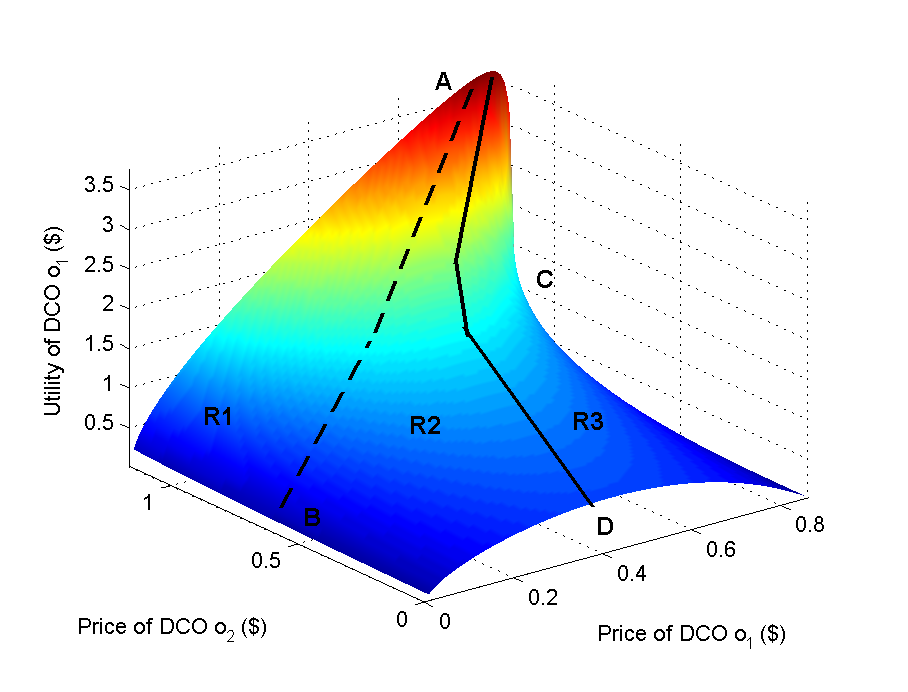
\includegraphics[scale=0.5, bb=479 262 86 558]{show_utilityDCO1_vs_prices.eps}
        \caption{Utility of DCO $o_1$ with different prices set by DCOs}
        \label{fig:DCO 1}\vspace{0.5 cm}
    \end{subfigure}
    \begin{subfigure}[b]{0.5\textwidth}
        \centering
        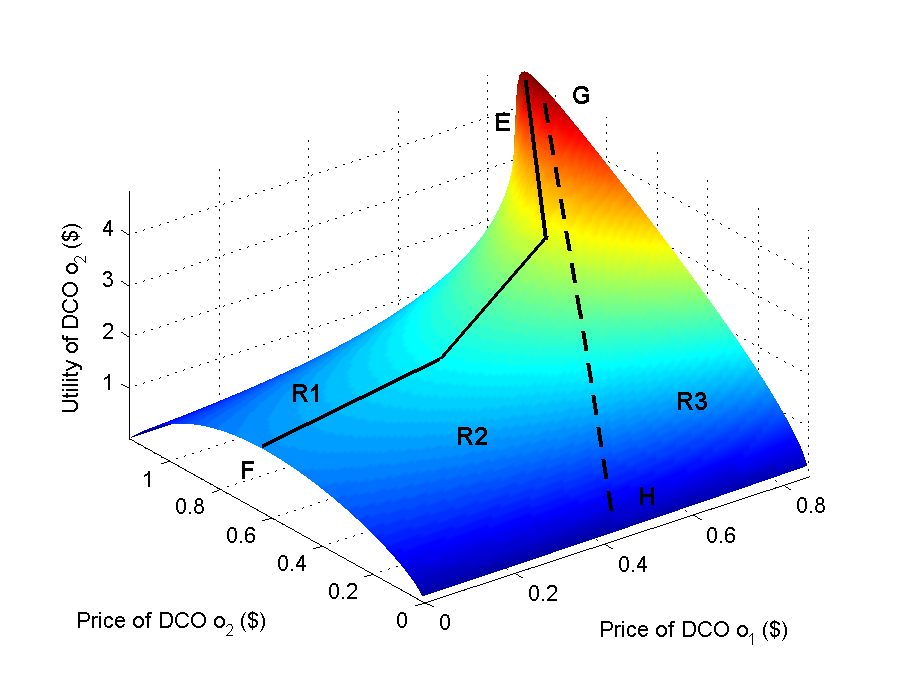
\includegraphics[scale=0.5, bb=479 262 86 558]{show_utilityDCO2_vs_prices.eps}
        \caption{Utility of DCO $o_2$ with different prices set by DCOs}
        \label{fig:DCO 2}
    \end{subfigure}
    \caption{Utilities of the DCOs with different pricing behaviors}
    \label{fig:dco_vs_prices}\vspace{-0.2 cm}
\end{figure}


With different prices, the utilities of both DCOs are shown in Fig. \ref{fig:dco_vs_prices}. When the price of DCO $o_2$ is fixed and DCO $o_1$ increases its service price, the probability for the SSs to choose DCO $o_1$ unilaterally decreases, but the utility of DCO $o_1$ firstly increases and then decreases. Similarly, when the price of DCO $o_1$ is fixed and DCO $o_2$ increases its service price, the utility of DCO $o_2$ firstly increases, then decreases. In order to better analyze the problem, we separate the figures into three regions.

\begin{enumerate}
  \item [R1] In the region 1, the price of DCO $o_2$ is relatively high, while the price of DCO $o_1$ is relatively low. Because of the large gap in price between both DCOs, even though DCO $o_2$ with a higher price is able to serve SSs with a lower delay and better performance, both SSs still prefer to choose DCO $o_1$, considering the total cost of the service. Accordingly, in order to serve the SSs and receive the highest revenues given strategies of the others, there are tradeoffs for both DCOs when they set their service prices. For DCO $o_2$, setting a high price allows it to receive high payment from serving the SSs. However, it should avoid setting a price far higher than that of DCO $o_1$. Otherwise, the probabilities for the SSs to choose DCO $o_2$ are low, and DCO $o_2$ cannot gain high revenues. For DCO $o_1$, setting low prices may help it serve more SSs, and receive more revenues. Nevertheless, as the service price is low, even though the amount of payment from SSs to DCO $o_1$ is large, DCO $o_1$ can only achieve limited revenue from a single SS. In general, the DCO may not receive high revenues.



  \item [R2] The price set by both DCOs at each point in this region is competitive. Accordingly, neither of the DCOs is able to be chosen by both SSs, and each DCO will serve one SS at the same time. In this situation, as the prices of both DCOs are competitive and each DCO needs to predict the behavior of the other DCO, and to set their serving prices optimally. On one hand, if the DCO is setting a price that is too high, its served SS will leave the service, resulting in a low revenue for the DCO. On the other hand, if the DCO sets a low price for its served SS, although the SS stays, the revenue of serving the SS is not maximized.

\item [R3] In region 3, the price of DCO $o_1$ is relatively high, while the price of DCO $o_2$ is relatively low. With the same reason as in the case of region 1, even though DCO $o_1$ with a higher price is able to serve the SSs with a lower delay and better performance, both SSs still prefer to choose DCO $o_2$, considering the total costs of the service. Therefore, on one hand, with prediction and estimation of the prices from DCO $o_2$, DCO $o_1$ should avoid setting the price that is too high falling into the region 3. On the other hand, DCO $o_2$ should compare and evaluate the total revenues, balancing the expected number of served SSs and setting a price.

\end{enumerate}

Therefore, when setting the price for the SSs, there is the competition between DCO $o_1$ and DCO $o_2$. Either DCO should estimate the behavior of the others, balance the setting price and number of the expected SSs and make decisions so as to achieve high revenues. In the general situation with $M$ DCOs and $N$ SSs, the figures become $M+1$ dimensions, which can be separated into $M+1$ regions. In each region, the tradeoff among DCOs' decisions works in a similar way.

However, for each DCO in the game, it is hard to predict the behaviors of other DCOs, causing unstable and unsatisfying results for each other. In the following sections, based on the different benefits of the SSs and DCOs, we propose both the competitive and the coordinated strategies for the DCOs to achieve the highest utility given the actions of other DCOs. In the real situations where some DCOs coordinate with some other DCOs, and some still compete with other DCOs, the DCOs that can cooperate with each other will coordinated with each other first. Then, each coordinated DCOs can be regarded as a coalition and compete with other DCOs outside of the coalition using the competitive algorithm.



\vspace{0.5 cm}

\subsubsection{The competitive behavior among DCOs}

In the noncooperative scenario where each DCO only considers its own revenue, in order to regulate the behaviors of the DCOs and obtain a stable and optimal solution, we propose a sub-gradient algorithm for DCOs of the game.

When DCOs adopt the sub-gradient algorithm, each DCO initially assumes that there is no competition with other DCOs and sets its service price at the maximum value to receive high utility. When the DCO discovers that there exist other DCOs trying to attract SSs with lower prices, the DCO predicts the reactions of the other DCOs on its own price and the tradeoff on its pricing strategy should be considered. If the DCO decreases its service price and competes with other DCOs, SSs are more likely to be served by the DCO. Thus, the expected number of served SSs increases. However, because of the low service price, the revenue the DCO obtain from each SS decreases. Similarly, when the DCO increases its service price, even though the DCO receives higher revenues from each served SS, as other DCOs serve SSs with lower prices and good performance, the number of SSs choosing the DCO decreases. Accordingly, in order to make optimal decisions based on the prediction other DCOs' strategies, we propose an iterated process for the DCOs to adjust their behaviors so as to receive optimal utilities. At each iteration, the DCO tries to increase or decrease its price with a small step and predict the resulting utility, if the adjustment increases its utility, the DCO will increase or decrease its price in the next iteration. Otherwise, the DCO will keep the current service price unchanged. Within finite number of iterations, all DCOs are able to determine the best decisions with the highest utilities. We assume that $\mathbf{p}=\langle p_{i} \rangle$ is the pricing profile of all DCOs in the previous iteration, $\mathbf{p}_{old}=\langle {p}_{old_i} \rangle$ is the pricing profile of all DCOs in the previous iteration, and $\mathbf{p}_{old_{-i}}$ is the pricing profile of all DCOs except DCO $o_i$ in the previous iteration. Accordingly, the detailed algorithm is shown as in Algorithm \ref{algorithm1}. Then, the following Lemma \ref{lemma2} holds for the proposed algorithm.




\begin{algorithm}[htb]
\caption{Strategy of each DCO in a multi-DCO multi-SS scenario.}
%\label{alg:background}
\vspace{.1cm}
\hrule
\begin{algorithmic}[1]
\vspace{.2cm}
        \STATE Initially, each DCO ignores the existence of other DCOs, and sets its price at the maximum value to receive the highest revenue from all SSs.
        \WHILE{at least one DCO adjusts its price}
        \FOR{SS $s_j$}
            \STATE Based on the prices set by all DCOs, each SS determines the probability to be served by each DCO and purchases the optimal amount of resource blocks from each DCO.
        \ENDFOR
         \FOR{DCO $o_i$}
            \STATE Each DCO stores the current value of service prices. $\mathbf{p}_{old}=\mathbf{p};$
            \STATE Each DCO adjusts its price with a small step $\Delta_i$ and calculate its own payoff based on the prediction of the followers' optimal strategies.
            \IF {$u_i({p}_{old_i}, \mathbf{p}_{old_{-i}})\leq u_i({p}_{old_i}+\Delta_i, \mathbf{p}_{old_{-i}})$}
                \STATE  $p_i=\min\{ p^{max}_i, p_{old_i}+\Delta_i\};$    \% Increase the price
            \ELSE
                \IF {$u_i({p}_{old_i}, \mathbf{p}_{old_{-i}})\leq u_i({p}_{old_i}-\Delta_i, \mathbf{p}_{old_{-i}})$}
                    \STATE  $p_i=\max \{ 0, p_{old_i}-\Delta_i\};$      \% Reduce the price
                \ELSE
                    \STATE  $p_i=p_{old_i};$  \% Keep the price unchanged
                \ENDIF
            \ENDIF
         \ENDFOR
         \ENDWHILE
\end{algorithmic}\label{algorithm1}
\hrule
\end{algorithm}



\begin{lemma} \label{lemma2}
When the starting price and step size of DCO $o_i$ $\Delta_i$, $\forall i \in \{1,2,\ldots,M\}$ are fixed, the game can always converge to a unique outcome, which is also the Nash equilibrium of the game.
\end{lemma}
\begin{proof}
The proof is provided in Appendix B. \end{proof}


\vspace{0.5 cm}

For the proposed sub-gradient algorithm, it is not necessary for all the players to be strictly synchronized when they make decisions. More specifically, for each SS, based on the observation of the announced prices from all DCOs, each SS determines the optimal amount of computing resource block to purchase. In this case, all the SSs do not have to make decisions at the exactly same time. For each DCO, based on the observation of the announced prices of other DCOs and the observation of current behaviors of all SSs, it is able to follow our proposed algorithm to set its price to improve its utility. In other words, all the DCOs also do not need to make decisions at the same time, and the algorithm can still converge to the same Stackelberg equilibrium.

Based on the results of the iterated approaches, the computing resource blocks are allocated afterwards. Therefore, the utilities or revenues received by all DCOs and SSs follow the results of the iterated approaches. After one period, all the DCOs will perform the sub-gradient algorithm and do the resource allocation again. Therefore, for the iterative approach ahead of one period, the resulting Nash Equilibrium is still an equilibrium solution for a static game, not dynamic one.


\subsubsection{Coalition formation in DCOs}

Even though all DCOs are able to achieve Nash equilibrium outcomes with the proposed sub-gradient algorithm, the revenue of each DCO is still low due to the competition with all other DCOs. To improve their benefits, DCOs may seek to cooperate with each other and jointly decide the price offered to the SSs. Accordingly, in the upper layer of multi-leader multi-follower hierarchical game, we propose the coalition game among all DCOs, in order to improve the utilities of the DCOs. However, some DCOs may be unwilling to cooperate with each other because of the unfair results within the coalition. We evaluate the capability of served SSs for each DCO as the revenue that the DCO receives when all the other DCOs stop serving SSs. Therefore, in order to guarantee fairness and avoid the competition among all DCOs in the coalition game, each DCO should set its price in the feasible region and obtain revenue proportional to its capability. In order to achieve the fair results and high revenues for all DCOs in the coalition game, we consider the Kalai-Smorodinsky bargaining as a resource division approach within all DCOs.



\begin{definition} \cite{HPark01}\cite{Huaqing01} \label{definition2}
We denote $\mathbf{U}=[u_{1},u_{2},\ldots, u_{M}]^\top$ as the feasible utility set, and let $\mathbf{h}=[h_{1},h_{2},\ldots, h_{M}]^\top$ be the disagreement point set, which are the expectations of operators by joining the game without cooperation. $\mathbf{Y}^*=F(\mathbf{U},\mathbf{h})$ is regarded as a Kalai-Smorodinsky bargaining solution if the following six axioms, i.e., individual rationality, feasibility, pareto optimality, individual monotonicity, independence of linear transformations, and symmetry, are satisfied.
\end{definition}




According to the conclusions of \cite{JChen01} and \cite{CZhang01}, $u^*=[u_{1}^*,u_{2}^*,\ldots,u_{M}^*]^\top$ can be a unique solution satisfying all axioms in Definition \ref{definition2}, if the solution meets the following condition

\begin{equation}
    \frac{{{\text{u}}_{1}^* -  {{h_{1}}} }}{{{\text{u}}_{1}^{\max } -  {{h_{1}}} }} = \frac{{{\text{u}}_{2}^* -  {{h_{2}}} }}{{{\text{u}}_{2}^{\max } -  {{h_{2}}} }} = \ldots = \frac{{{\text{u}}_{M}^* -  {{h_{M}}} }}{{{\text{u}}_{M}^{\max } -  {{h_{M}}} }},
\end{equation}
where ${{u}}_{i}^{\max }$, $\forall i \in \{1,2,\ldots,M\}$, is the maximum utility of DCO $o_i$ when all SSs are served by the DCO $o_i$ with the highest price $p^{max}_i$, i.e.,

\begin{equation}
    {{u}}_{i}^{\max }= \sum\limits_{j = 1}^N {u^{max}_{ij}},
\end{equation}
where

\begin{equation}
u^{max}_{ij}=\left( {\frac{{{\lambda _j}}}{{{\mu _i}}}\sqrt {p_i^{\max }}  + \frac{{{\lambda _j}}}{{{\mu _i}}}p_i^{\max } - c{\beta _{ij}}\frac{{{\lambda _j}}}{{{\mu _i}\sqrt {p_i^{\max }} }} - c{\beta _{ij}}\frac{{{\lambda _j}}}{{{\mu _i}}}} \right).
\end{equation}

When all DCOs are noncooperative, the DCOs compete with each other by reducing their prices. Accordingly, we suppose that in the competition, the corresponding utility of each DCO $o_i$ is zero, i.e., $h_i=0$, $\forall i \in \{1,2,\ldots,M\}$ \cite{Huaqing01}.


Based on the utilities of DCOs, we have the following lemma.

\vspace{0.2 cm}

\begin{lemma} \label{theorem2}
For each DCO $o_{i}$ in the coalition formation, $\forall i \in \{1,2,\ldots,M\}$, when all DCOs adopt Kalai-Smorodinsky bargaining as a resource division approach, the setting price of the DCO $o_{i}$ satisfies

\begin{equation}
    p_{i}^*= {\left({p_{i}^{\max }} \right)}^ -,
\end{equation}
where $\left({\cdot}\right)^-$ approaches the limit from the negative side. Correspondingly, the utility of each DCO $o_i$, $\forall i \in \{1,2,\ldots,M\}$ is

\begin{equation}
    u_i^*= {\sum\limits_{j = 1}^N \frac{1}{N}{u^{max}_{ij}} },
\end{equation}
where
\begin{equation}
u^{max}_{{i}j}={\frac{{{\lambda _j}}}{{{\mu _{i}}}}\sqrt {p_{i}^{\max }}  + \frac{{{\lambda _j}}}{{{\mu _{i}}}}p_{i}^{\max } - c{\beta _{{i}j}}\frac{{{\lambda _j}}}{{{\mu _{i}}\sqrt {p_{i}^{\max }} }} - c{\beta _{{i}j}}\frac{{{\lambda _j}}}{{{\mu _{i}}}}}.
\end{equation}


\end{lemma}
\begin{proof}
The proof is provided in Appendix C. \end{proof}

\vspace{0.5 cm}


\section{Simulation Results and Discussions}\label{sec:simulations}




In this section, we present the simulations to evaluate the performances of the proposed approaches with MATLAB. Without loss of generality, we follow the settings in \cite{ZLiu01} and assume that there are two DCOs accessible to three SSs at the same time. We set the service rate of each computing resource block in both DCOs as $0.3$ $(ms)^{-1}$. The workload arrival rates for SS $s_1$, SS $s_2$ and SS $s_3$ are $0.7$ $(ms)^{-1}$, $0.6$ $(ms)^{-1}$, and $0.6$ $(ms)^{-1}$, respectively. We model the distance between source and data center, divided by the transmission
speed of $200 km/ms$, resulting in delay ranging in $[0, 8]$ ms, and the delay tolerance of all SSs is set to $8$ ms. The above settings are reasonable for the existing data center networks. \cite{ZLiu01} In the proposed sub-gradient method, we assume that the price step sizes for both DCOs are $0.01$ dollar.


In Fig. \ref{fig:rth_vs_social}, we compare our proposed sub-gradient algorithm with the ordinary noncooperative behavior where each DCO sets its optimal price based on the observation of other DCOs' behaviors in the previous iteration. The noncooperative behavior cannot guarantee the convergence of the game. In the simulation, we performed $1000$ iterations and took the average of 10 latest results as an expected social welfare value. Moreover, we compare the proposed algorithm with the cooperative behavior, where each DCO can increase its served price regardless of the number of served SSs. Accordingly, in order to achieve the high utilities for all DCOs, each DCO sets its price as the maximum possible value. In our proposed Kalai-Smorodinsky bargaining method, both DCOs form a coalition with each other based on the bargaining strategy to achieve fair revenues. The social welfare achieved by the Kalai-Smorodinsky bargaining follows the results of cooperative behaviors. As shown in Fig. \ref{fig:rth_vs_social}, with the increased delay tolerance $r_{th}$ of SSs, all DCOs are able to set a high price to meet the service requirements of the SSs, and the performance of the SSs deteriorates. Therefore, the social welfare generally reduces with $r_{th}$ increasing. Furthermore, at each value of $r_{th}$, the social welfare is always higher than the expected social welfare of the noncooperative strategy when the DCOs adopt the proposed sub-gradient algorithm. The social welfare when both DCOs are cooperative is the lowest, because when the DCOs cooperate with each other, even though the DCOs receive high revenues, all SSs suffer more because of the high service price and low quality of service. Based on the above results, from the perspective of SSs or the management of data center services, in order to achieve high social welfare, both DCOs should compete with each other, and the proposed sub-gradient algorithm is a good tool to achieve stable and high revenues.

\begin{figure}[!t]
\centering
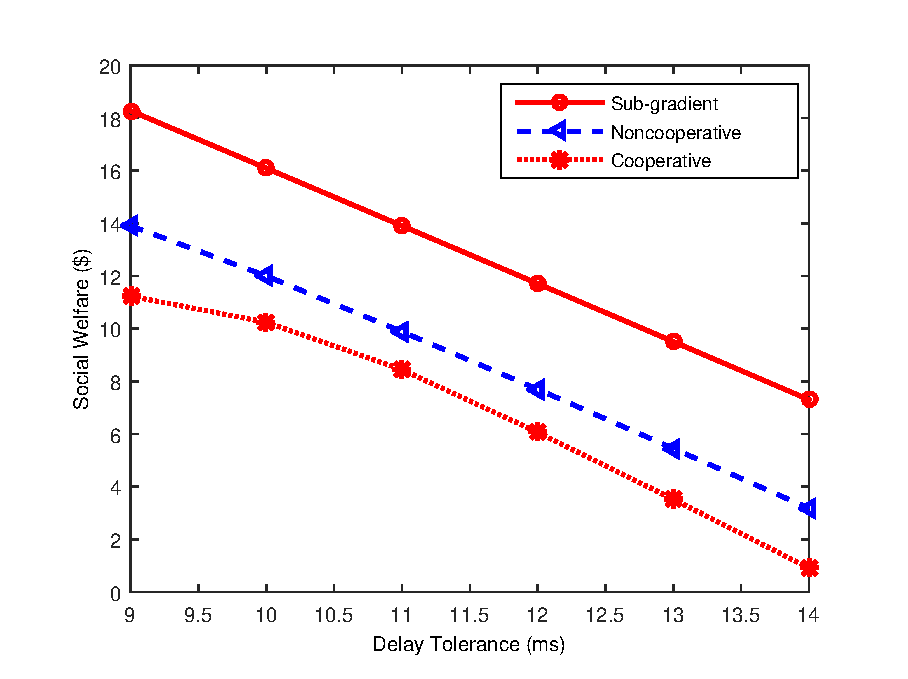
\includegraphics[scale=0.45, bb=391 0 18 299]{fig_rth_social.eps}
\caption{Social welfare vs delay tolerance of SSs with different approaches}
\label{fig:rth_vs_social}
\end{figure}


From the perspective of DCOs, the situation is different. In Fig. \ref{fig:utilitydco}, we compare the utility of each DCO in coalition formation with Kalai-Smorodinsky bargaining, noncooperative scenario with sub-gradient algorithm, ordinary noncooperative behavior, and the situation where only DCO $o_1$ or DCO $o_2$ monopolizes the market. As shown in Fig. \ref{fig:utilitydco}, we discover that when the DCOs form a coalition and adopt Kalai-Smorodinsky bargaining, the utilities of both DCOs are higher than the utilities when DCOs employ the proposed sub-gradient strategy or take the noncooperative behaviors. As both DCOs form a coalition, they do not need to compete with each other in order to achieve high revenues. They set their prices at high values to increase the total utilities for the DCOs so as to obtain high utilities through bargaining. The utilities of both DCOs when adopting the proposed sub-gradient strategy are also higher than the utilities in noncooperative behaviors. Furthermore, we discover in the single DCO situation, where all SSs have no choice on their serving DCOs, the DCO is able to receive higher utility than that when there are multiple DCOs. However, compared with the proposed Kalai-Smorodinsky bargaining strategy, it is hard to coordinate one DCO to give up all its services to the other DCO if only one DCO serves the SSs, and the quality of service of SSs is lower.

\begin{figure}[!t]
\centering
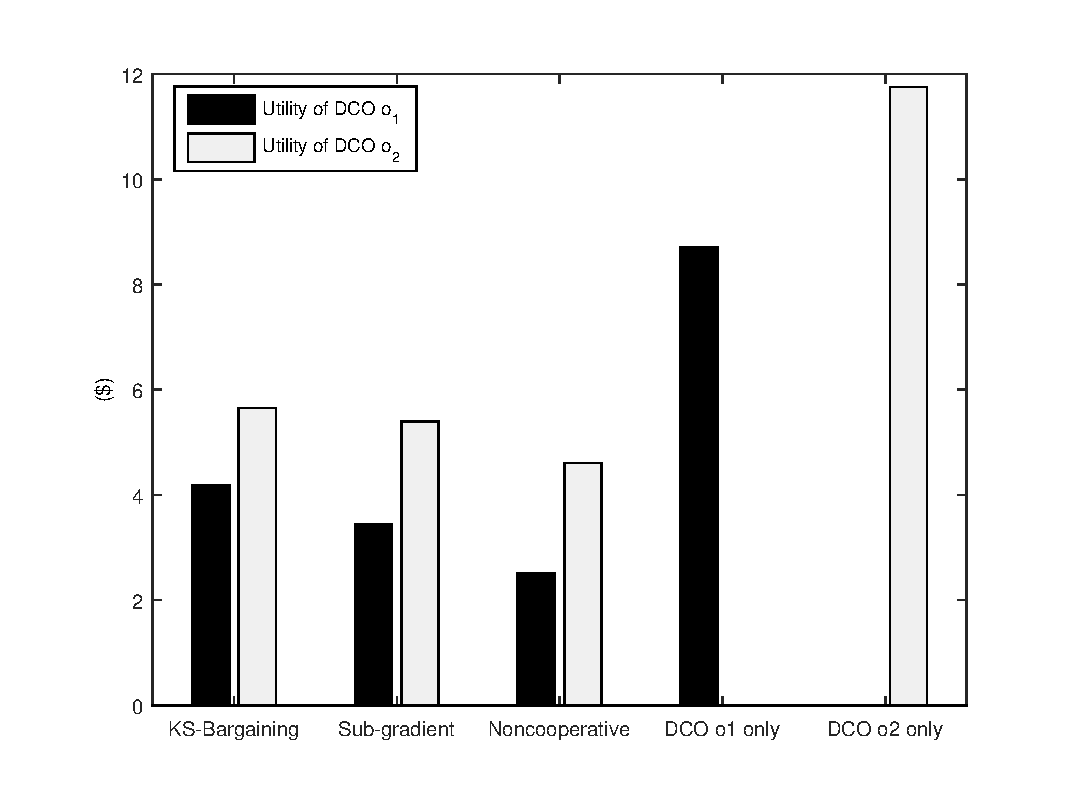
\includegraphics[scale=0.42, bb=466 15 34 359]{fig2_utilityDCO.eps}
\caption{The utility of each DCO with different approaches}
\label{fig:utilitydco}
\end{figure}

In Fig. \ref{fig:step}, we evaluate the impact of the step size in the proposed sub-gradient strategy. In the simulation, we fix the step size of DCO $o_2$ as $0.01$, and change the step size of DCO $o_1$ to $0.005$, $0.01$, $0.015$, $0.02$, respectively. According to the algorithm of the proposed sub-gradient strategy, with a different step size of DCO $o_1$, both DCOs compete with each other and gradually reduce their prices in the game. The game finally converges to the similar results, within different range to the same sub-optimal point of the game. Furthermore, when the step size increases, with the same starting point, the convergence speed of the corresponding DCO is faster, but the range of the sub-optimal point increases. As the starting price of the proposed sub-gradient strategy is the maximum possible value of each DCO, we discover that when the step size increases, the service price of the DCO after convergence is higher, causing a lower utility for its served SSs. Therefore, there is a tradeoff for the SSs' choices. When the step size is large, the convergence time of service is small, but the gap between the optimal value and achieved value is large. When the step size is small, the gap between the achieving value and the optimal value is small, but the delay is large because of the slow convergence time with sub-gradient algorithm. Accordingly, if the SSs is more sensitive to the time delay of the service, it may require fast convergence of the DCO's strategies. However, the DCO may be able to set higher prices for the SSs for higher utilities. On the other hand, if the SSs expect lower prices from the DCO, the SSs may prefer a small step size of the DCO and tolerate higher convergence time in order to purchase the services with optimal prices.



\begin{figure}[!t]
\centering
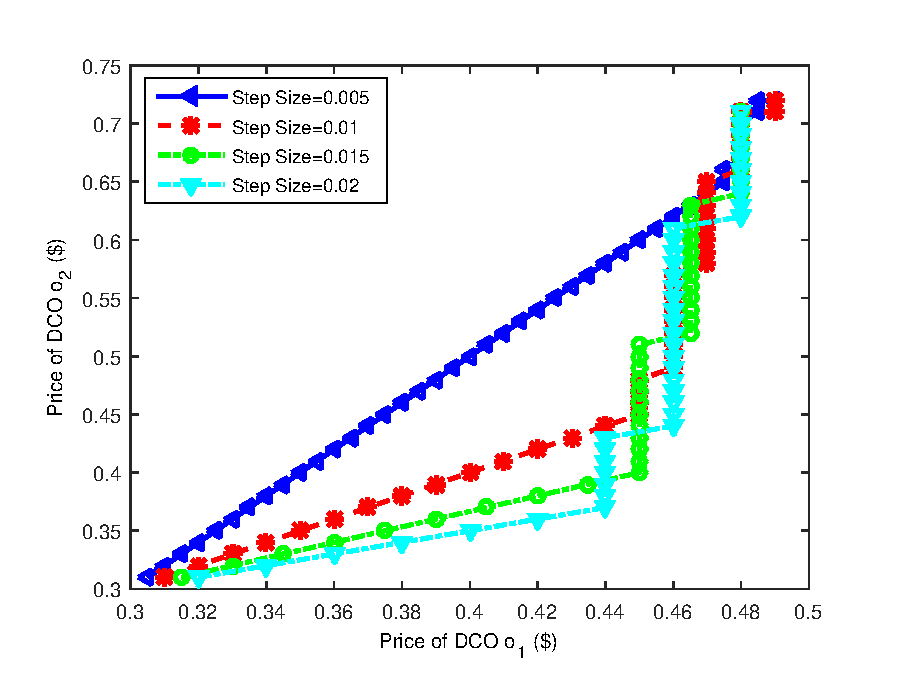
\includegraphics[scale=0.45, bb=391 0 13 302]{fig_step_route.eps}
\caption{The converge route in the proposed sub-gradient strategy with different steps}
\label{fig:step}
\end{figure}




In Fig. \ref{fig:lambda} and Fig. \ref{fig:miu}, we evaluate the impacts of the workload requirements of SSs and the service rates of both DCOs, respectively, for the proposed sub-gradient strategy. As shown in Fig. \ref{fig:lambda}, without loss of generality and for better presentation, we fix the workload requirements of SS $s_3$ as $0.6$ Mbps and consider the utility of DCO $o_1$ with different workload values of SSs $s_1$ and $s_2$. When we consider the same workload value of SS $s_1$ (or $s_2$) and increase the workload value of SS $s_2$ (or $s_1$), DCO $o_1$ is able to serve SS $s_2$ (or $s_1$) with more computing resources, so the utility of DCO $o_1$ increases, even though there is the competition between the DCOs. In Fig. \ref{fig:miu}, we consider the performance of $SS$ $s_1$ with different service rate of both DCOs. When the service rates of both DCOs are small, even though the delay of the service is large for $SS$ $s_1$, both DCOs set low prices for the service, and the utility of SS $s_1$ reaches the maximum value. However, when both DCOs increase their service rate simultaneously, the DCOs set higher prices for the service of SS $s_1$. Accordingly, the utility of SS $s_1$ decreases. Moreover, when DCO $o_1$ (or DCO $o_2$) has a low service rate, but DCO $o_2$ (or DCO $o_1$) improves its service rate, the utility of SS $s_1$ first increases and then decreases. Because when the service rate of DCO $o_1$ (or DCO $o_2$) is low, its price is set at a low value. When DCO $o_2$ (or DCO $o_1$) improves its service rate, because of the competition of both DCOs, the utility of SS $s_1$ first increases because of the low price and high quality of service. However, when DCO $o_2$ (or DCO $o_1$) continues to improve its service rate, DCO $o_1$ (or DCO $o_2$) also increases its price to receive high utility. Therefore, the utility of $SS$ $s_1$ decreases.



\begin{figure}[!t]
\centering
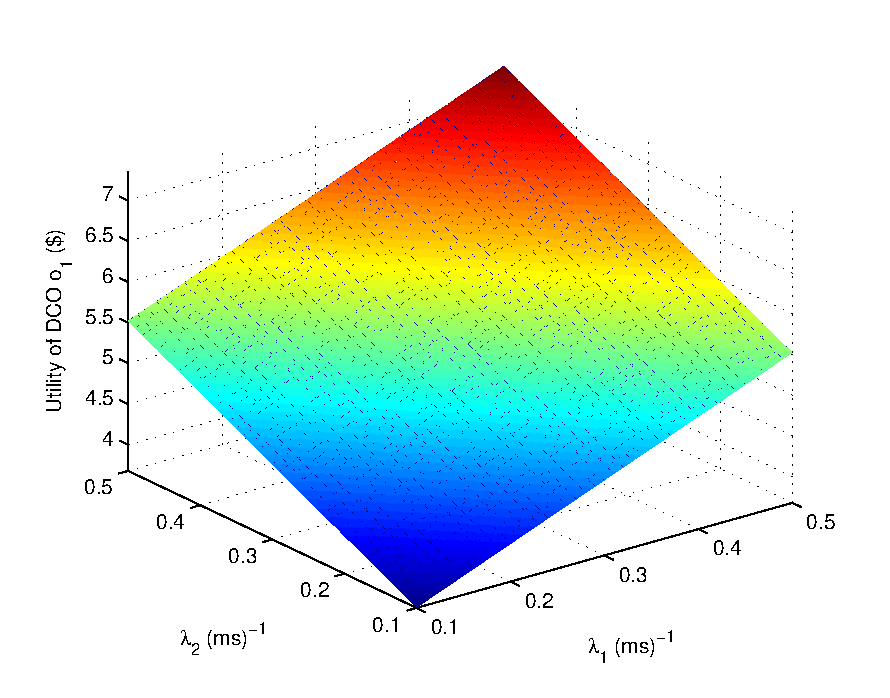
\includegraphics[scale=0.45, bb=490 265 95 564]{fig_lam_vs_dco.eps}
\caption{Utility of DCO $o_1$ vs the workload requirements of SS $s_1$ and SS $s_2$}
\label{fig:lambda}
\end{figure}


\begin{figure}[!t]
\centering
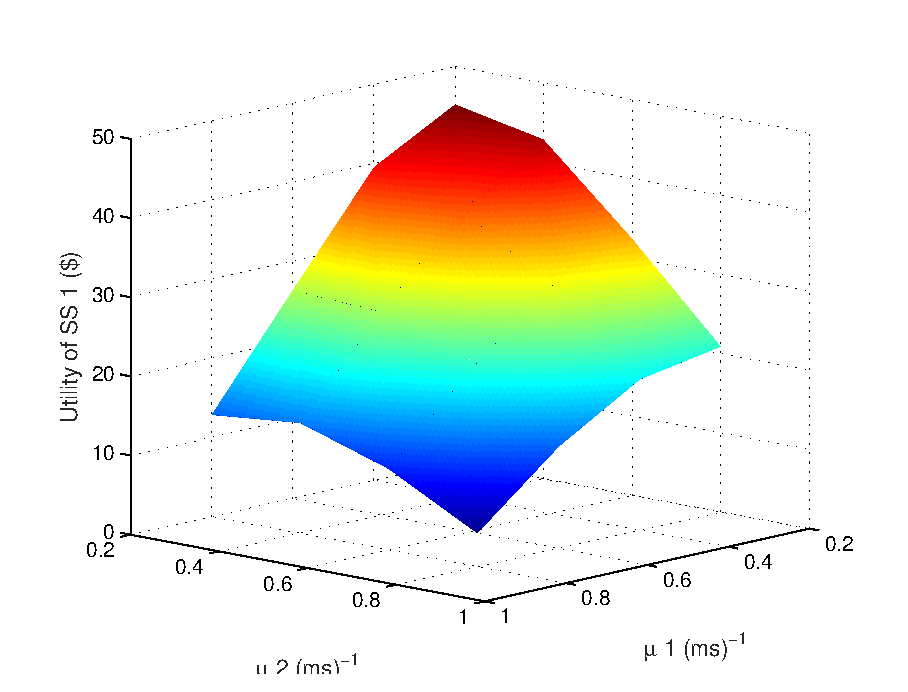
\includegraphics[scale=0.45, bb=493 253 99 558]{fig_miu_vs_ss.eps}
\caption{Utility of SS $s_1$ vs the service rate of both DCOs}
\label{fig:miu}
\end{figure}


\section{Related works}\label{sec:related}

The resource allocation problem has been widely studied for data center networking systems. \cite{Mastelic01} performed a comprehensive analysis of energy efficiency in a general infrastructure supporting the cloud computing paradigm. The authors first defined a systematic approach for analysis, then utilized the approach to analyze data centers and finally extracted existing challenges and future works. In \cite{Wang01}, the authors overviewed data center networks for cloud computing and evaluate construction prototypes for future works in order to improve the agility for multi-tenant demands in the cloud, responsiveness and scalability.

Specifically, in \cite{LGu01}, the authors studied various problems for large-scale data centers including task assignment, data placement, and data movements. An optimization algorithm that could minimize the total cost during the big data computing services was proposed. To ensure all users to efficiently and securely share the network resources, authors in \cite{TWang01} evaluated the performance of several popular network sharing policies, such as SecondNet \cite{CGuo01}, Oktopus \cite{HBallani01}, Gatekeeper \cite{HRodrigues01}, Seawall \cite{AShieh01}, NetShare \cite{TLam01}, and FairCloud \cite{LPopa01}, in a data center with multiple users. In \cite{JZhang01}, the authors showed a class of data center network structures based on hypergraph theory and combinatorial block design theory. Compared with the classic fat-tree model, the new structures of constructing large data center networks are more flexible and scalable. In \cite{YShang01}, the authors made comprehensive comparison study for typical data center networks with regard to their Network Power Effectiveness (NPE). The results showed that Flattened Butterfly \cite{JKim01} network topology achieved high NPE in most of the cases, and the NPE of the server-centric architectures was usually higher than the NPEs of Fat-Tree \cite{CELeiserson01} and VL2 \cite{AGreenberg01} architectures.

In order to reduce the power consumption of network elements, the authors in \cite{YZhang01} designed a two-level, pod-level, and core-level power optimization model, namely, Hierarchical EneRgy Optimization (HERO). The HERO optimized the way of shutting down network switches and links while guaranteeing full connectivity and maximizing link utilization of the network. A novel framework was proposed in \cite{LWang01}, where high energy efficiency could be achieved by assigning virtual machines to servers and reducing the number of active switches and balance traffic flows. In order to achieve high energy efficiency, the authors in \cite{LWang02}, took advantage of the application characteristics and topology features and proposed TE-VMA and TER algorithms to assign virtual machines and routing traffic flows, respectively. In \cite{ZShu01}, a novel architecture of Cloud-integrated Cyber-Physical System was proposed and the enabling technologies for Complex Industrial Applications (CIA) was outlined. The paper provided solutions for the virtualized resource management techniques, the scheduling of cloud resources and life cycle management from the perspective of CIA. In \cite{LWang03}, the authors focused on the performance-guaranteed energy-saving schemes. Based on the constraint that the transmission of every flow has to be accomplished before a rigorous deadline, the authors explored the most energy efficient way of scheduling and routing flows on the network, as well as determining the transmission speed for every flow. \cite{Polverini01} explored the benefit of electricity price variations across time and locations for the data centers. The authors proposed a GreFar algorithm to optimizes the energy cost and fairness among different organizations subject to queueing delay and maximum server inlet temperature constraints. In \cite{Wei01}, the authors considered a QoS-constrained resource allocation problem with game theory. In the game, each participant first solved its optimization problem with binary integer programming. Then an evolutionary mechanism was designed to consider the relationships of different participants and minimize their efficiency losses. In \cite{Ren01}, the authors considered the adaptive and stable application deployment in clouds with a multi-objective evolutionary game-theoretic framework. In the proposed framework, resource allocation strategy to applications was analyzed based on the location and the operational conditions in a cloud.

In \cite{LLiu01}, the authors considered the efficiency of water usage, and optimized a framework for the workload management of data centers. In order to design a new, upgraded and expanded data center network, the authors in \cite{ARCurtis01} proposed a data center network design framework. By searching the space of all networks that are feasible under a user-specified data center model, the proposed framework maximized bisection bandwidth and minimized end-to-end latency of the designed network. In \cite{CJChen01}, the authors analyzed the management problem of data centers with multiple layers or heterogeneous devices. A new simulation tool, called Data Center Simulator with small scale operating system and storage, was proposed.

\section{Conclusions and Future Work}\label{sec:conclusion}

In this paper, we have studied the resource allocation problem when multiple data center operators (DCOs) and service subscribers (SSs)    coexist in the networks. In order to analyze the relationships among multiple DCOs and SSs, we have modeled the scenario as a multi-leader multi-follower hierarchical game, where the DCOs act as leaders and the SSs act as followers. With the prediction of behaviors of all SSs and reactions of other DCOs, we have discussed the utilities of the DCOs in different situations and proposed the sub-gradient algorithm in the noncooperative game and coalition game with Kalai-Smorodinsky bargaining strategies to gain the benefits in terms of social welfare and the utilities of the DCOs, respectively. Simulation results have demonstrated that for the benefits of SSs, all DCOs compete with each other and all DCOs adopt the proposed sub-gradient strategies to achieve high social welfare of the game. On the other hand, for the benefits of DCOs, DCOs form a coalition and perform Kalai-Smorodinsky bargaining behaviors so as to achieve high and fair revenues. The game analysis of the relationship between DCOs and SSs provides an outlook for the future work in the multi-DCO multi-SS scenarios. Future work is in progress to consider the resource allocation problem including both the massive and edge data center networks.

\section*{Appendix A: Proof of Lemma~\ref{theorem1}}
\begin{proof}
As the cost of the SS is continuous, we take the second derivative of $v_{1}$ with respect to $m_{11}$,

\begin{equation}
   \frac{{{\partial ^2}{v_{1}}}}{{\partial m_{11}^2}} =  - \frac{{2\lambda _{1}^2{\mu _1}}}{{{{({\mu _1}{m_{11}} - {\lambda _{1}})}^3}}}.
\end{equation}

Since the second derivative of $v_{1}$ with respect to $m_{11}$ is less than zero, $v_{1}$ is a concave function of $m_{11}$. By setting the first derivative of $v_{1}$ with respect to $m_{11}$ as zero, i.e.,

\begin{equation}
   \frac{{\partial {v_{1}}}}{{\partial {m_{11}}}} = {\left( {\frac{{\lambda _{1}}}{{{\mu _1}{m_{11}} - {\lambda _{1}}}}} \right)^2} - {p_1} = 0,
\end{equation}
we can obtain the optimal strategy for the SS, which is given by,

\begin{equation}
    m_{11}^*=\frac{{{\lambda _{1}}}}{{{\mu _1}\sqrt {{p_1}} }} + \frac{{{\lambda _{1}}}}{{{\mu _1}}}.
\end{equation}
\end{proof}

\section*{Appendix B: Proof of Lemma~\ref{lemma2}}
\begin{proof}
The convergence of the sub-gradient algorithm has been proved in \cite{SPBoyd} and \cite{YXiao01}.

According to \cite{SPBoyd} and \cite{YXiao01}, the sub-gradient algorithm is able to achieve a sub-optimal solution with small ranges. Therefore, with a given moving step size, each DCO is unable to unilaterally adjust its price in order to receive higher utility when the sub-gradient algorithm converges to a sub-optimal solution.

Furthermore, when the starting price and step size $\Delta_i$, $\forall i \in \{1,2,\ldots,M\}$ are fixed, the results in the second iteration are fixed. According to the mathematical induction, we suppose that at the $Q^{th}$ iteration, the prices of both DCOs are fixed. Then in the $(Q+1)^{th}$ iteration, according to the proposed sub-gradient algorithm, the step size is fixed and the direction from the current iteration to the next iteration is unique. Therefore, the prices of both DCOs in the $(Q+1)^{th}$ iteration are also fixed. Therefore, based on the above, the game can converge to a unique outcome, when the starting price and step size $\Delta_i$, $\forall i \in \{1,2,\ldots,M\}$ are fixed. \end{proof}






\section*{Appendix C: Proof of Lemma~\ref{theorem2}}
\begin{proof}
According to the definition of Kalai-Smorodinsky bargaining, the optimal prices for DCOs $\mathbf{p}^*=[{p_1}^*,{p_2}^*,\ldots,{p_M}^*]^\top$  satisfy


\begin{equation}\label{optinks}
    \begin{array}{l}
     \begin{gathered}
 \mathbf{p}^* = \arg \max {\kern 1pt} \,{\text{u}}_{1}^* \hfill\\
  s.t.  {\begin{array}{*{20}{l}}
  {\frac{{{\text{u}}_{1}^*  }}{{{\text{u}}_{1}^{\max }  }} = \frac{{{\text{u}}_{2}^*  }}{{{\text{u}}_{2}^{\max } }} = \ldots = \frac{{{\text{u}}_{M}^*  }}{{{\text{u}}_{M}^{\max }  }}}.
\end{array}}  \hfill
\end{gathered}
    \end{array}
\end{equation}

When the prices offered by the DCOs satisfy

\begin{equation}
    p_{i}= {\left({p_{i}^{\max }} \right)}^ -,
\end{equation}
the corresponding utility of each DCO $o_i$, $\forall i \in \{1,2, \ldots, M\}$, is

\begin{equation}
    u_i= {\sum\limits_{j = 1}^N \frac{1}{N}{u^{max}_{ij}} },
\end{equation}
where

\begin{equation}
u^{max}_{{i}j}={\frac{{{\lambda _j}}}{{{\mu _{i}}}}\sqrt {p_{i}^{\max }}  + \frac{{{\lambda _j}}}{{{\mu _{i}}}}p_{i}^{\max } - c{\beta _{{i}j}}\frac{{{\lambda _j}}}{{{\mu _{i}}\sqrt {p_{i}^{\max }} }} - c{\beta _{{i}j}}\frac{{{\lambda _j}}}{{{\mu _{i}}}}}.
\end{equation}

Furthermore, as the maximum utility of each DCO $o_i$, $\forall i \in \{1,2, \ldots, M\}$, equals

\begin{equation}
    {{u}}_{i}^{\max }= \sum\limits_{j = 1}^N {u^{max}_{ij}},
\end{equation}
where

\begin{equation}
u^{max}_{ij}=\left( {\frac{{{\lambda _j}}}{{{\mu _i}}}\sqrt {p_i^{\max }}  + \frac{{{\lambda _j}}}{{{\mu _i}}}p_i^{\max } - c{\beta _{ij}}\frac{{{\lambda _j}}}{{{\mu _i}\sqrt {p_i^{\max }} }} - c{\beta _{ij}}\frac{{{\lambda _j}}}{{{\mu _i}}}} \right).
\end{equation}
We discover

\begin{equation}
{\frac{{{\text{u}}_{1}  }}{{{\text{u}}_{1}^{\max }  }} = \frac{{{\text{u}}_{2}  }}{{{\text{u}}_{2}^{\max } }} = \ldots = \frac{{{\text{u}}_{M}  }}{{{\text{u}}_{M}^{\max }  }}} = \frac{1}{N}.
\end{equation}

According to the utility function of each DCO $o_i$, $\forall i \in \{1,2,\ldots,M\}$, $u_i$ is monotonically increasing with the improvement of $p_i$. Therefore, when $p_i$ approaches its maximum value, the corresponding utility of DCO $o_i$ can also achieve the highest value. The highest utility of DCO $o_i$ follows the constraint in (\ref{optinks}). Accordingly, when the price of DCO $o_{i}$ is

\begin{equation}
    p_{i}^*= {\left({p_{i}^{\max }} \right)}^ -,
\end{equation}
the utility of each DCO $o_i$, $\forall i \in \{1,2,\ldots,M\}$ achieves

\begin{equation}
    u_i^*= {\sum\limits_{j = 1}^N \frac{1}{N}{u^{max}_{ij}} }.
\end{equation} \end{proof}








%%%



\begin{thebibliography}{1}
\bibitem{AGreenberg02}
A. Greenberg, J. Hamilton, D. A. Maltz, P. Patel, ``The cost of a cloud: research problems in data center networks,'' {\em \it ACM SIGCOMM Computer Comm. Review,} vol. 39, no. 1, pp. 68-73, Jan. 2009.


\bibitem{Amazon01}
Amazon Web Service, available at ``http://aws.amazon.com''.

\bibitem{Google01}
Google app engine, available at ``http://code.google.com/appengine/''.

\bibitem{Google02}
Google docs and spreadsheets, available at ``http://docs.google.com''.

\bibitem{Microsoft01}
Microsoft office live, available at ``http://office.live.com''.

\bibitem{Microsoft02}
Windows Azure, available at ``http://www.microsoft.com/azure/''.

\bibitem{Yahoo01}
Yahoo! Mail, available at ``http://mail.yahoo.com''.

\bibitem{Mastelic01}
T. Mastelic, A. Oleksiak, H. Claussen, I. Brandic, J.-M. Pierson and A. V. Vasilakos, ``Cloud computing: Survey on energy efficiency,''{\em \it ACM Computing Surveys (CSUR),} vol. 47, no. 2, pp. 1-36, Jan. 2015.

\bibitem{Wang01}
B. Wang, Z. Qi, R. Ma, H. Guan and A. V. Vasilakos. ``A survey on data center networking for cloud computing,''{\em \it Computer Networks,} vol. 91, pp. 528-547, Nov. 2015.

\bibitem{LGu01}
L. Gu, D. Zeng, P. Li, and S. Guo, ``Cost minimization for big data processing in geo-distributed data centers,'' {\em \it IEEE Trans. Emerging Topics in Computing,} vol. 2, no. 3, pp. 314-323, Sep. 2014.

\bibitem{TWang01}
T. Wang, Z. Su, Y. Xia and M. Hamdi, ``Rethinking the data center networking: architecture, network protocols, and resource sharing,'' {\em \it IEEE Access,} vol. 2, pp. 1481-1496, Dec. 2014.

\bibitem{CGuo01}
C. Guo, G. Lu, H. J. Wang, S. Yang, C Kong, P. Sun, W. Wu, and Y. Zhang, ``SecondNet: A data center network virtualization architecture with bandwidth guarantees,'' in {\em \it Proc. 6th Int'l COnference (Co-NEXT'10),} Philadelphia, PA, Dec. 2010.

\bibitem{HBallani01}
H. Ballani, P. Costa, T. Karagiannis, and A. Rowstron, ``Towards predictable datacenter networks,'' in {\em \it Proc. ACM SIGCOMM'11,} vol. 41, no. 4, pp. 242-253, Toronto, Canada, Aug. 2011.


\bibitem{HRodrigues01}
H. Rodrigues, J. R. Santos, Y. Turner, P. Soares, and D. Guedes, ``Gatekeeper: Supporting bandwidth guarantees for multi-tenant datacenter networks,'' in {\em \it Proc. USENIX WIOV,} Portland, OR, Jun. 2011.

\bibitem{AShieh01}
A. Shieh, S. Kandula, A. Greenberg, C. Kim, and B. Saha, ``Sharing the data center network,'' in {\em \it  Proc. 8th USENIX Conf. Netw. Syst. Design Implement (NSDI),} pp. 309-322, Boston, MA, Mar. 2011.

\bibitem{TLam01}
T. Lam, and G. Varghese, ``NetShare: Virtualizing bandwidth within the cloud,'' {\em \it  UCSD Technical Report}, 2009.

\bibitem{LPopa01}
L. Popa, A. Krishnamurthy, S. Ratnasamy, and I. Stoica, ``FairCloud: Sharing the network in cloud computing,'' in {\em \it Proc. ACM SIGCOMM Conf. Applications, Technologies, Architectures, and Protocols for Computer Comm.,} pp. 187-198, Helsinki, Finland, Aug. 2012.


\bibitem{JZhang01}
J. Zhang, Z. Fang, G. Qu, and S. Q. Zheng, ``A new class of data center network structures,'' in {\em \it Proc. IEEE Globecom'13,} Atlanta, GA, Dec. 2013.

\bibitem{YShang01}
Y. Shang, D. Li, J. Zhu, and M. Xu, ``On the network power effectiveness of data center architectures,'' {\em \it IEEE Trans. Computers,} vol. 64, no. 11, pp. 3237-3248, Nov. 2015.



\bibitem{JKim01}
J. Kim, W. J. Dally, and D. Abts ``Flattened butterfly: a cost-efficient topology for high-radix networks,'' {\em \it ACM SIGARCH Computer Architecture News,} vol. 35, no. 2, pp. 126-137, Jun. 2007.

\bibitem{CELeiserson01}
C. E. Leiserson, ``Fat-trees: Universal Networks for Hardware-Efficient
Supercomputing,'' {\em \it IEEE Trans. Computers,} vol. 34 , no. 10,
pp. 892-901, Oct. 1985.

\bibitem{AGreenberg01}
A. Greenberg, J. R. Hamilton, N. Jain, S. Kandula, C. Kim, P. Lahiri, D. A. Maltz, P. Patel, and S. Sengupta, ``VL2: A scalable and flexible data center network,'' {\em \it Comm. of the ACM,} vol. 54, no. 3, pp. 95-104, Mar. 2011.

\bibitem{YZhang01}
Y. Zhang, and N. Ansari, ``HERO: Hierarchical energy optimization for data center networks,'' {\em \it IEEE Systems Journal,} vol. 9, no. 2, pp. 406-415, Jun. 2015.


\bibitem{LWang01}
L. Wang, et al, ``GreenDCN: A General Framework for Achieving Energy Efficiency in Data Center Networks,''{\em \it in IEEE Journal on Selected Areas in Communications,} vol. 32, no. 1, pp. 4-15, Jan. 2014.

\bibitem{LWang02}
L. Wang, F. Zhang, A. V. Vasilakos, C. Hou and Z. Liu, ``Joint virtual machine assignment and traffic engineering for green data center networks,''{\em \it SIGMETRICS Perform. Eval. Rev.,} vol. 41, no. 3, pp. 107-112, Jan. 2014.

\bibitem{ZShu01}
Z. Shu, J. Wan, D. Zhang and D. Li, ``Cloud-integrated cyber-physical systems for complex industrial applications,''{\em \it Mobile Networks and Applications,} pp. 1-14, Nov. 2015

\bibitem{LWang03}
L. Wang, F. Zhang, K. Zheng, A. V. Vasilakos, S. Ren and Z. Liu, ``Energy-Efficient Flow Scheduling and Routing with Hard Deadlines in Data Center Networks,''{\em \it Distributed Computing Systems (ICDCS), 2014 IEEE 34th International Conference on,} pp. 248-257, Madrid, Spain, Jun. 2014.

\bibitem{Polverini01}
M. Polverini, A. Cianfrani, S. Ren and A. V. Vasilakos, ``Thermal-Aware Scheduling of Batch Jobs in Geographically Distributed Data Centers,''{\em \it in IEEE Transactions on Cloud Computing,} vol. 2, no. 1, pp. 71-84, Mar. 2014.

\bibitem{Wei01}
G. Wei, A. V. Vasilakos, Y. Zheng and N. Xiong, ``A game-theoretic method of fair resource allocation for cloud computing services,''{\em \it The journal of supercomputing,} vol. 54, no. 2, pp. 252-269, Nov. 2010.

\bibitem{Ren01}
Y. Ren, J. Suzuki, C. Lee, A. V. Vasilakos, S. Omura and K. Oba, ``Balancing performance, resource efficiency and energy efficiency for virtual machine deployment in DVFS-enabled clouds: an evolutionary game theoretic approach,''{\em \it Proceedings of the Companion Publication of the 2014 Annual Conference on Genetic and Evolutionary Computation. ACM,} pp. 1205-1212, Vancouver, Canada, Jul. 2014.


\bibitem{LLiu01}
L. Liu, S. Ren, and Z. Han, ``Scalable workload management for water efficiency in data centers,'' in {\em \it Proc. IEEE Globecom'14,} Austin, TX, Dec. 2014.


\bibitem{ARCurtis01}
A. R. Curtis, T. Carpenter, M. Elsheikh, A. L-. Ortiz, and S. Keshav, ``REWIRE: An optimization-based framework for unstructured data center network design,'' in {\em \it Proc. IEEE INFOCOM'12,} Orlando, FL, Mar. 2012.


\bibitem{CJChen01}
C.-J. Chen, Y.-S. Liu, and R.-G. Chang, ``DCSim: Design analysis on virtualization data center,'' in {\em \it Proc.  9th Int'l Conf. Ubiquitous Intelligence and Computing and  Autonomic and Trusted Computing (UIC/ATC),} Fukuoka, Japan, Sep. 2012.

\bibitem{ECaron01}
E. Caron, F. Desprez, D. Loureiro, and A. Muresan, ``Cloud computing resource management through a grid middleware: A case study with DIET and Eucalyptus,'' in {\em \it Proc. IEEE Int'l Conf.  Cloud Computing 2009,} pp. 151-154, Bangalore, India, Sep. 2009.

\bibitem{AGan01}
A. Gandhi, M. Harchol-Balter, R. Das, and C. Lefurgy, ``Optimal power allocation in server farms,'' {\em \it ACM SIGMETRICS Perform. Eval. Rev.,} vol. 37, no. 1, pp. 157-168, Jun. 2009.



\bibitem{ZLiu01}
Z. Liu, M. Lin, A. Wierman, S. H. Low, and L. L. Andrew, ``Geographical load balancing with renewables,'' {\em \it ACM SIGMETRICS Perform. Eval. Rev.,} vol. 39, no. 3, pp. 62-66, Dec. 2011.

\bibitem{SRen01}
S. Ren and Y. He, ``COCA: Online distributed resource management for cost minimization and carbon neutrality in data centers,'' in {\em \it Proc. ACM Int'l Conference on High Performance Computing, Networking, Storage and Analysis,} Denver, CO, Nov. 2013.

\bibitem{hzhang12}
H. Zhang, M. Bennis, L. A. DaSilva and Z. Han, ``Multi-leader Multifollower Stackelberg Game among Wi-Fi, Small Cell and Macrocell Networks,'' {\em \it IEEE Global Communications Conference,} pp. 4520-4524, Austin, TX, Dec. 2014.

\bibitem{YChen}
Y. Chen, J. Zhang, and Q. Zhang, ``Utility-aware refunding framework for hybrid access femtocell network,'' {\em \it IEEE Trans. Wireless Comm.,} vol. 11, no. 5, pp. 1688-1697, May 2012.

\bibitem{HuaqingR01}
H. Zhang, M. Bennis, L. A. DaSilva and Z. Han, ``Multi-leader multi-follower stackelberg game among Wi-Fi, small cell and macrocell networks,'' {\em \it 2014 IEEE Global Communications Conference,} pp. 4520-4524, Austin, TX, Dec. 2014.


\bibitem{HPark01}
H. Park and M. Schaar, ``Fairness strategies for multi-user multimedia applications in competitive environments using the kalai-smorodinsky bargaining solution,'' in {\em \it Proc. IEEE Int'l Conf. Acoustics, Speech and Signal Processing (ICASSP)'07,} Honolulu, HI, Apr. 2007.

\bibitem{Huaqing01}
H. Zhang, Y. Xiao, L. X. Cai, D. Niyato, L. Song, and Z. Han,``A hierarchical game approach for multi-operator spectrum sharing in LTE unlicensed,'' in  {\em \it Proc. IEEE Globecom'15,} San Diego, CA, Dec. 2015.



\bibitem{JChen01}
J. Chen and A. L. Swindlehurst, ``Downlink resource allocation for multi-user MIMO-OFDMA systems: The Kalai-Smorodinsky bargaining approach,'' in {\em \it Proc. IEEE Int'l Workshop Computational Advances in Multi-Sensor Adaptive Processing (CAMSAP)'09,} Aruba, Dutch Antilles, Netherlands, Dec. 2009.

\bibitem{CZhang01}
C. Zhang and H. Zhao, ``A novel fair cooperation strategy based on Kalai-Smorodinsky bargaining solution for selfish cooperative relay networks,'' in {\em \it Proc. IEEE Int'l Conf. Intelligent Transportation Systems (ITSC)'14,} pp. 2107-2112, Qingdao, China, Oct. 2014.

\bibitem{SPBoyd}
S. P. Boyd and L. Vandenberghe, {\em ``Convex Optimization,''  Cambridge
University Press,} 2004.

\bibitem{YXiao01}
Y. Xiao, G. Bi, and D. Niyato, ``A simple distributed power control algorithm for cognitive radio networks,'' {\em \it IEEE Trans. Wireless Comm.,} vol. 10, no. 11, pp. 3594-3600, Nov. 2011.



\end{thebibliography}


\begin{IEEEbiography}[{
\includegraphics[width=1in,height=1.25in,clip,keepaspectratio]{Huaqing.eps}}]{Huaqing Zhang} (M'14) received the B.S. degree in Huazhong University of Science and Technology, Wuhan, China, in June 2013. He is now pursuing the Ph.D. degree in the department of electronic and computer engineering at University of Houston, Houston, TX, USA. He has been a reviewer for TWC, TCCN, TBC, and JWCN. His research interest includes wireless communications and networking, zero-determinant strategy, and hierarchical game.
\end{IEEEbiography}

\begin{IEEEbiography}[{
\includegraphics[width=1in,height=1.25in,clip,keepaspectratio]{XiaoYong.eps}}]{Yong Xiao}(S'09-M'13-SM'15) received his B.S. degree in electrical engineering from China University of Geosciences, Wuhan, China in 2002, M.Sc. degree in telecommunication from Hong Kong University of Science and Technology in 2006, and his Ph. D degree in electrical and electronic engineering from Nanyang Technological University, Singapore in 2012. From August 2010 to April 2011, he was a research associate in school of electrical and electronic engineering, Nanyang Technological University, Singapore. From May 2011 to October 2012, he was a research fellow at CTVR, school of computer science and statistics, Trinity College Dublin, Ireland. From November 2012 to December 2013, he was a postdoctoral fellow at Massachusetts Institute of Technology. From December 2013 to November 2014, he was a MIT-SUTD postdoctoral fellow with Singapore University of Technology and Design and Massachusetts Institute of Technology. From November 2014 to August 2015, he was a postdoctoral fellow II at Department of Electrical and Computer Engineering at University of Houston. Currently, he is a research assistant professor in the Department of Electrical and Computer Engineering at the University of Arizona. He is also the center manager of the NSF BWAC Center at the University of Arizona. His research interests include machine learning, game theory and their applications in communication networks. He is an IEEE senior member.
\end{IEEEbiography}


\begin{IEEEbiography}[{\includegraphics[width=1in,height=1.25in,clip,keepaspectratio]{Bu.eps}}]{Shengrong Bu} received the PhD degree in electrical and computer engineering from Carleton University in 2012, and held a research position at Huawei Technologies Canada Inc. Ottawa as a NSERC IRDF until 2014. She is now a Lecturer (Assistant Professor equivalent) with the School of Engineering at the University of Glasgow, Scotland. Her research interests include energy-efficient networks, smart grids, big data analytics, wireless networks, wireless network security, cloud computing, game theory and stochastic optimization. She received three best paper awards at IEEE International conferences. Highlights of her professional activities include duties as an editor for IEEE TCGCC NewsLetters, an associate editor for the journal Springer Wireless Networks, TPC co-chair for six international workshops or conference symposiums, and duties as N2Women mentoring Co-Chair. She has sat on the TPC for more than twenty leading international conferences and workshops and served as a reviewer for more than ten leading journals.
\end{IEEEbiography}


\begin{IEEEbiography}[{
\includegraphics[scale=0.2, bb=340 0 0 463]{Yu.eps}}]{F. Richard Yu}(S��00-M��04-SM��08) received the PhD degree in electrical engineering from the University of British Columbia (UBC) in 2003. From 2002 to 2006, he was with Ericsson (in Lund, Sweden) and a start-up in California, USA. He joined Carleton University in 2007, where he is currently a Professor. He received the IEEE Outstanding Service Award in 2016, IEEE Outstanding Leadership Award in 2013, Carleton Research Achievement Award in 2012, the Ontario Early Researcher Award (formerly Premiers Research Excellence Award) in 2011, the Excellent Contribution Award at IEEE/IFIP TrustCom 2010, the Leadership Opportunity Fund Award from Canada Foundation of Innovation in 2009 and the Best Paper Awards at IEEE ICC 2014, Globecom 2012, IEEE/IFIP TrustCom 2009 and Int'l Conference on Networking 2005. His research interests include cross-layer/cross-system design, security, green ICT and QoS provisioning in wireless-based systems.

He serves on the editorial boards of several journals, including Co-Editor-in-Chief for Ad Hoc \& Sensor Wireless Networks, Lead Series Editor for IEEE Transactions on Vehicular Technology, and IEEE Transactions on Green Communications and Networking, IEEE Communications Surveys \& Tutorials. He has served as the Technical Program Committee (TPC) Co-Chair of numerous conferences. Dr. Yu is a registered Professional Engineer in the province of Ontario, Canada, and a senior member of the IEEE. He serves as a member of Board of Governors of the IEEE Vehicular Technology Society.

\end{IEEEbiography}


\begin{IEEEbiography}[{
\includegraphics[width=1in,height=1.25in,clip,keepaspectratio]{Dusit_Niyato.eps}}]{Dusit Niyato}(M'09-SM'15) is currently an Associate Professor in the School of Computer Science and Engineering, at Nanyang Technological University, Singapore. He received B.Eng. from King Mongkuts Institute of Technology Ladkrabang (KMITL) in 1999 and Ph.D. in Electrical and Computer Engineering from the University of Manitoba, Canada in 2008. His research interests are in the area of energy harvesting for wireless communication, Internet of Things (IoT) and sensor networks.
\end{IEEEbiography}



\begin{IEEEbiography}[{
\includegraphics[width=1in,height=1.25in,clip,keepaspectratio]{Han.eps}}]{Zhu Han} (S'01-M'04-SM'09-F'14) received the B.S. degree in electronic engineering from Tsinghua University, in 1997, and the M.S. and Ph.D. degrees in electrical and computer engineering from the University of Maryland, College Park, in 1999 and 2003, respectively.

From 2000 to 2002, he was an R\&D Engineer of JDSU, Germantown, Maryland. From 2003 to 2006, he was a Research Associate at the University of Maryland. From 2006 to 2008, he was an assistant professor at Boise State University, Idaho. Currently, he is a Professor in the Electrical and Computer Engineering Department as well as in the Computer Science Department at the University of Houston, Texas. His research interests include wireless resource allocation and management, wireless communications and networking, game theory, big data analysis, security, and smart grid. Dr. Han received an NSF Career Award in 2010, the Fred W. Ellersick Prize of the IEEE Communication Society in 2011, the EURASIP Best Paper Award for the Journal on Advances in Signal Processing in 2015, IEEE Leonard G. Abraham Prize in the field of Communications Systems (best paper award in IEEE JSAC) in 2016, and several best paper awards in IEEE conferences. Currently, Dr. Han is an IEEE Communications Society Distinguished Lecturer.
\end{IEEEbiography}



\end{document}

%-------------------------------------------




